\documentclass{beamer}
\usepackage{graphicx}
\usepackage{xcolor}
\usepackage{tikz}
\usepackage{amsmath}
\usepackage{pgfplots}
\pgfplotsset{compat=1.18}

\definecolor{purpleblue}{RGB}{80, 80, 180}
\definecolor{novelPurple}{RGB}{98, 54, 255}
\definecolor{softPurple}{RGB}{180, 170, 255}
\definecolor{softGray}{RGB}{235, 235, 245}
\definecolor{lightText}{RGB}{90, 90, 110}

\usetheme{Madrid}
\usecolortheme{dolphin}
\graphicspath{{static/course_materials/}{static/hard/}{./}}

\setbeamerfont{title}{size=\Large,series=\bfseries}
\setbeamerfont{frametitle}{size=\LARGE,series=\bfseries}
\setbeamercolor{frametitle}{fg=white, bg=novelPurple}
\setbeamercolor{title}{fg=white, bg=purpleblue}

\title[Test III]{\textbf{Test III}}
\author{\textbf{Jack Zeng}}
\institute{\textcolor{white}{\textbf{Novel Prep}}}
\date{\today}

\begin{document}

\begin{frame}
    \titlepage
    \vfill
    \begin{flushright}
        \textcolor{purpleblue}{\Huge \textbf{Novel Prep}}
    \end{flushright}
\end{frame}

\begin{frame}
    \begin{tikzpicture}[remember picture, overlay]
        \shade[top color=softPurple, bottom color=softGray]
            (current page.north west) rectangle (current page.south east);
        \node[align=center] at (current page.center) {
            {\Huge\bfseries\textcolor{purpleblue}{Novel Prep}} \\[0.5cm]
            {\Large\itshape\textcolor{lightText}{Phase 3 · Mock Exam Training}}
        };
    \end{tikzpicture}
\end{frame}

\begin{frame}{Overview}
    \tableofcontents
\end{frame}

\begin{frame}
\section{Test III}
    \begin{tikzpicture}[remember picture, overlay]
        \shade[top color=softPurple, bottom color=softGray]
            (current page.north west) rectangle (current page.south east);
        \node[align=center] at (current page.center) {
            {\LARGE\bfseries\textcolor{purpleblue}{Test III}} \\[0.5cm]
            {\Large\itshape\textcolor{lightText}{22 Module 2-style mock exam questions}}
        };
    \end{tikzpicture}
\end{frame}

% --- Question 1 ---
\begin{frame}{Question 1}
\small
A packaging engineer is optimizing a cardboard sleeve whose width profile is modeled by the quadratic expression \(ax^2 + 176x + c\), where \(a\) and \(c\) are positive constants. If \(px + q\) is a factor of the expression,
\[
ax^2 + 176x + c = (px + q)(rx + s),
\]
where \(p\) and \(q\) are positive constants, what is the greatest possible value of \(ac\)?
\end{frame}
\begin{frame}{Answer 1}
\small
\textbf{Final Answer:} $\boxed{7744}$
\end{frame}

% --- Question 2 ---
\begin{frame}{Question 2}
\small
A signal-processing filter uses a polynomial in the variable \(z^9\) to tune resonance. In the given expression,
\[
34z^{18} + b z^9 + 30,
\]
\(b\) is a positive integer. If \(qz^9 + r\) is a factor of the expression, where \(q\) and \(r\) are positive integers, what is the greatest possible value of \(b\)?
\end{frame}
\begin{frame}{Answer 2}
\small
\textbf{Final Answer:} $\boxed{1021}$
\end{frame}

% --- Question 3 ---
\begin{frame}{Question 3}
\small
An optics lab rewrites a focusing model into paired quadratic factors in \(x^2\). The expression
\[
6x^4 + 17x^2 + 7
\]
can be rewritten as \((3x^2 + a)(2x^2 + b)\), where \(a\) and \(b\) are positive integers, or as \((3x^2 + c)(2x^2 + d)\), where \(c\) and \(d\) are positive non-integers.

What is the value of \(a + c\)?
\end{frame}
\begin{frame}{Answer 3}
\small
\textbf{Final Answer:} $\boxed{\dfrac{17}{2}}$
\end{frame}

% --- Question 4 ---
\begin{frame}{Question 4}
\small
A materials scientist factors a stiffness polynomial before running a simulation. The given quadratic function
\[
54x^4 + 219x^2 + 105
\]
has factors in the form \((k)(ax^2 + b)(cx^2 + d)\). If \(a, b, c, d, k\) are integers, what is the smallest possible value of \(ab\)?
\end{frame}
\begin{frame}{Answer 4}
\small
\textbf{Final Answer:} $\boxed{14}$
\end{frame}

% --- Question 5 ---
\begin{frame}{Question 5}
\small
A drone’s altitude path over a short flight is modeled by a parabola in the \(xy\)-plane. The equation of a parabola is written in the form
\[
y = ax^2 + bx + c,
\]
where \(a, b, c\) are constants. When graphed in the \(xy\)-plane, the parabola has vertex \((-1, 4)\) and does not intersect the \(x\)-axis. Which of the following could be the value of \(a - b - c\)?
\vspace{0.35cm}
\begin{enumerate}
    \item[A.] \(2\)
    \item[B.] \(4\)
    \item[C.] \(-1\)
    \item[D.] \(-6\)
\end{enumerate}
\end{frame}
\begin{frame}{Answer 5}
\small
\textbf{Correct Answer:} D
\end{frame}

% --- Question 6 ---
\begin{frame}{Question 6}
\small
A fountain’s water arc is modeled by a downward-opening quadratic with vertex \((1, 32)\). A quadratic function with vertex \((1, 32)\) can be written as
\[
 -ax^2 + bx + c \quad (a, b, c \text{ are all positive integers}).
\]
What is the maximum value of \(b\)?
\end{frame}
\begin{frame}{Answer 6}
\small
\textbf{Final Answer:} $\boxed{62}$
\end{frame}

% --- Question 7 ---
\begin{frame}{Question 7}
\small
A robotics team measures that a test cart’s speed is increasing at a rate of \(7.7\ \text{meters per second squared}\). What is this rate in \textbf{miles per minute squared}, rounded to the nearest tenth? (Use \(1\ \text{mile} = 1609\ \text{meters}\).)
\vspace{0.35cm}
\begin{enumerate}
    \item[A.] \(0.3\)
    \item[B.] \(17.2\)
    \item[C.] \(206.5\)
    \item[D.] \(209\)
\end{enumerate}
\end{frame}
\begin{frame}{Answer 7}
\small
\textbf{Correct Answer:} B
\end{frame}

% --- Question 8 ---
\begin{frame}{Question 8}
\small
A bacteria culture in a bioreactor is modeled by an exponential growth function. The function \(f\) is defined by
\[
f(x) = ab^{x/n},
\]
where \(a, b, n\) are constants, and \(b, n\) are integers. If \(f(2) = 6\) and \(f(4) = 150\), what is the value of \(f(5)\)?
\end{frame}
\begin{frame}{Answer 8}
\small
\textbf{Final Answer:} $\boxed{750}$
\end{frame}

% --- Question 9 ---
\begin{frame}{Question 9}
\small
A roller-coaster design uses a parabolic track segment \(y = f(x)\). The graph of \(y = f(x)\) in the \(xy\)-plane has a vertex at \((4, -7)\), contains the point \((3, -9)\), and has a \(y\)-intercept at \((0, a)\). The graph of \(y = 6 \cdot f(x)\) has a \(y\)-intercept at \((0, b)\). What is the positive difference between \(a\) and \(b\)?
\end{frame}
\begin{frame}{Answer 9}
\small
\textbf{Final Answer:} $\boxed{195}$
\end{frame}

% --- Question 10 ---
\begin{frame}{Question 10}
\small
An economist fits a quadratic revenue model \(y = f(x)\) that breaks even at two production levels. The function \(f\) is defined by
\[
f(x) = ax^2 + bx + c,
\]
where \(a, b, c\) are constants. The graph of \(y = f(x)\) passes through the points \((9, 0)\) and \((-2, 0)\). If \(a\) is an integer greater than 1, which of the following could be the value of \(a + b\)?
\vspace{0.35cm}
\begin{enumerate}
    \item[A.] \(8\)
    \item[B.] \(7\)
    \item[C.] \(-6\)
    \item[D.] \(-12\)
\end{enumerate}
\end{frame}
\begin{frame}{Answer 10}
\small
\textbf{Correct Answer:} D
\end{frame}

% --- Question 11 ---
\begin{frame}{Question 11}
\small
A bridge support cable clearance is checked using polynomial factors in \(x\). Which of the following expressions has a factor of \(x + 2b\), where \(b\) is a positive integer constant?
\vspace{0.35cm}
\begin{enumerate}
    \item[A.] \(3x^2 + 7x + 14b\)
    \item[B.] \(3x^2 + 22x + 14b\)
    \item[C.] \(3x^2 + 30x + 14b\)
    \item[D.] \(3x^2 + 37x + 14b\)
\end{enumerate}
\end{frame}
\begin{frame}{Answer 11}
\small
\textbf{Correct Answer:} D
\end{frame}

% --- Question 12 ---
\begin{frame}{Question 12}
\small
A survey crew measures a triangular lot \(XYZ\) for a small park. In triangle \(XYZ\), the measure of angle \(Y\) is \(38^\circ\). The length of \(XY\) is 12 meters, and the length of \(YZ\) is 5 meters. What is the area, in square meters, of triangle \(XYZ\)?
\vspace{0.35cm}
\begin{enumerate}
    \item[A.] \(30\)
    \item[B.] \(60\)
    \item[C.] \(30 \sin 38^\circ\)
    \item[D.] \(60 \sin 38^\circ\)
\end{enumerate}
\end{frame}
\begin{frame}{Answer 12}
\small
\textbf{Correct Answer:} C
\end{frame}

% --- Question 13 ---
\begin{frame}{Question 13}
\small
A quality team selects two random samples to estimate the average lifespan of a street-lamp bulb (in hours). Based on the first sample, the estimated average lifespan is 800 hours, with a margin of error of 20 hours.

Based on the second sample, the estimated average lifespan is 810 hours, with a margin of error of 35 hours.

Assuming the margins of error were calculated in the same way, which of the following best explains why the first sample obtained a smaller margin of error than the second sample?
\vspace{0.35cm}
\begin{enumerate}
    \item[A.] The first sample contained fewer light bulbs than the second sample.
    \item[B.] The first sample contained more light bulbs than the second sample.
    \item[C.] The first sample had a shorter average lifespan than the second sample.
    \item[D.] The first sample had a longer average lifespan than the second sample.
\end{enumerate}
\end{frame}
\begin{frame}{Answer 13}
\small
\textbf{Correct Answer:} B
\end{frame}

% --- Question 14 ---
\begin{frame}{Question 14}
\small
A vibration model for a machine mount is given by a quartic that is written in shifted form. The function \(p(x)\) is defined by:
\[
p(x) = a((x - 3)^2 + b)((x - 3)^2 - c),
\]
where \(a, b,\) and \(c\) are constants. The graph of \(y = p(x)\) passes through the points \((1, 25)\) and \((-1, 52)\).

What is the value of \(p(5) + p(7)\)?
\vspace{0.35cm}
\begin{enumerate}
    \item[A.] \(25\)
    \item[B.] \(27\)
    \item[C.] \(52\)
    \item[D.] \(77\)
\end{enumerate}
\end{frame}
\begin{frame}{Answer 14}
\small
\textbf{Correct Answer:} D
\end{frame}

% --- Question 15 ---
\begin{frame}{Question 15}
\small
A savings balance is modeled by an exponential function of time. In the given function, \(b\) is a positive constant. For every increase in the value of \(x\) by 1, the value of \(f(x)\) increases by \(c\%\), where \(0 < c < 100\).

Which expression gives the value of \(c\) in terms of \(b\)?
\[
f(x) = 66(b)^x
\]
\vspace{0.35cm}
\begin{enumerate}
    \item[A.] \(1 + \dfrac{b}{100}\)
    \item[B.] \(b + 100\)
    \item[C.] \(100(b + 1)\)
    \item[D.] \(100(b - 1)\)
\end{enumerate}
\end{frame}
\begin{frame}{Answer 15}
\small
\textbf{Correct Answer:} D
\end{frame}

% --- Question 16 ---
\begin{frame}{Question 16}
\small
A park service tracks the average growth of a young oak. On average, a certain tree grows 87 centimeters every \(m\) months. At this rate, which expression represents the number of centimeters, on average, the tree grows every \(k\) years?
\vspace{0.35cm}
\begin{enumerate}
    \item[A.] \(\dfrac{29m}{4k}\)
    \item[B.] \(\dfrac{29k}{4m}\)
    \item[C.] \(\dfrac{1044m}{k}\)
    \item[D.] \(\dfrac{1044k}{m}\)
\end{enumerate}
\end{frame}
\begin{frame}{Answer 16}
\small
\textbf{Correct Answer:} D
\end{frame}

% --- Question 17 ---
\begin{frame}{Question 17}
\small
A circular plaza is being surveyed. In the figure shown, points \(A\), \(B\), \(C\), and \(E\) lie on the circle, and \(AB < BC\). Angle \(ABC\) is a right angle, segment \(AC\) is a diameter of the circle, and segment \(AC\) is perpendicular to segment \(BE\) at point \(D\). Also, \(BD = \sqrt{346}\). The diameter of the circle is 175. If \(\dfrac{CD}{AD} = r\), what is the value of \(r\)?

\begin{center}
    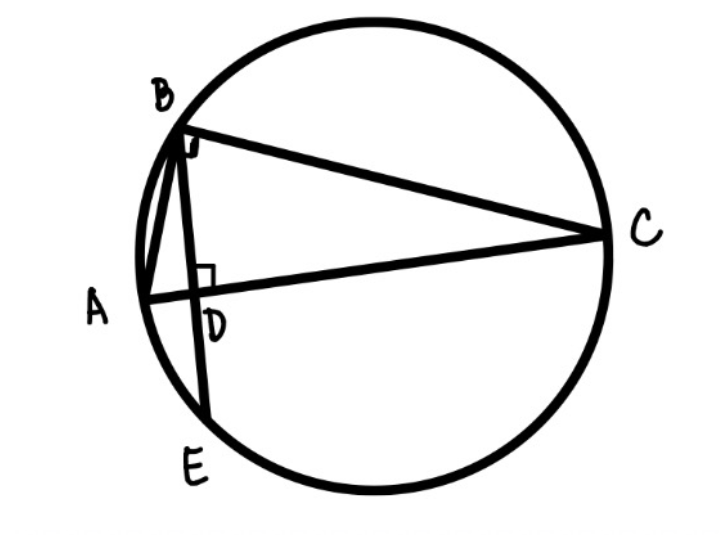
\includegraphics[width=0.48\linewidth]{hard_22_f2.png}
\end{center}
\end{frame}
\begin{frame}{Answer 17}
\small
\textbf{Final Answer:} $\boxed{86.5}$
\end{frame}

% --- Question 18 ---
\begin{frame}{Question 18}
\small
An engineer solves a timing equation before calibrating two sensors. In the given equation, \(a\) and \(k\) are constants, where \(k > 5a\). The sum of the solutions to the equation is \(3k + 32\). What is the value of \(a\)?
\[
(x - k)^2 = (k - 5a)(x - k)
\]
\vspace{0.35cm}
\begin{enumerate}
    \item[A.] \(-\dfrac{32}{5}\)
    \item[B.] \(\dfrac{32}{5}\)
    \item[C.] \(-\dfrac{5}{32}\)
    \item[D.] \(\dfrac{5}{32}\)
\end{enumerate}
\end{frame}
\begin{frame}{Answer 18}
\small
\textbf{Correct Answer:} A
\end{frame}

% --- Question 19 ---
\begin{frame}{Question 19}
\small
A lab predicts bacteria population (in thousands) with an exponential model. The equation \(N(m) = 63(Q)^{m/6}\) gives the predicted population \(N(m)\), in thousands, of a certain bacteria colony \(m\) minutes after the initial measurement, where \(Q\) is a constant greater than 1. The predicted population increases by \(p\%\) every 180 seconds.

What is the value of \(p\) in terms of \(Q\)?
\vspace{0.35cm}
\begin{enumerate}
    \item[A.] \(100(Q^{30} - 1)\)
    \item[B.] \(100(Q^{\frac{1}{2}} - 1)\)
    \item[C.] \(100(Q^{30} + 1)\)
    \item[D.] \(100(Q^{1.5} + 1)\)
\end{enumerate}
\end{frame}
\begin{frame}{Answer 19}
\small
\textbf{Correct Answer:} B
\end{frame}

% --- Question 20 ---
\begin{frame}{Question 20}
\small
A logistics planner solves an equation whose solutions represent two delivery windows. In the given equation, \(m\) and \(n\) are constants. The sum and product of the solutions of the equation are 8 and \(\dfrac{7}{2}\), respectively.

What is the value of \(\dfrac{m}{n}\)?
\[
(x - m)^2 = (m + 2n)(2x - n)
\]
\vspace{0.35cm}
\begin{enumerate}
    \item[A.] \(-\dfrac{1}{3}\)
    \item[B.] \(\dfrac{1}{3}\)
    \item[C.] \(-3\)
    \item[D.] \(3\)
\end{enumerate}
\end{frame}
\begin{frame}{Answer 20}
\small
\textbf{Correct Answer:} D
\end{frame}

% --- Question 21 ---
\begin{frame}{Question 21}
\small
A landscaping crew is staining a yard fence and must buy enough product for two coats. One gallon of stain will cover 170 square feet of a surface. A yard has a total fence area of \(w\) square feet.
Which equation represents the total amount of stain \(S\), in gallons, needed to stain the fence in this yard twice?
\vspace{0.35cm}
\begin{enumerate}
    \item[A.] \(S = \dfrac{w}{170}\)
    \item[B.] \(S = 170w\)
    \item[C.] \(S = 340w\)
    \item[D.] \(S = \dfrac{w}{85}\)
\end{enumerate}
\end{frame}
\begin{frame}{Answer 21}
\small
\textbf{Correct Answer:} D
\end{frame}

% --- Question 22 ---
\begin{frame}{Question 22}
\small
A projectile’s height in a scaled coordinate model is given by \(y = -x^2 + 9x - 100\). In the \(xy\)-plane, the graph of this equation intersects the line \(y = c\) at exactly one point. What is the value of \(c\)?
\vspace{0.35cm}
\begin{enumerate}
    \item[A.] \(-\dfrac{481}{4}\)
    \item[B.] \(-100\)
    \item[C.] \(-\dfrac{319}{4}\)
    \item[D.] \(-\dfrac{9}{2}\)
\end{enumerate}
\end{frame}
\begin{frame}{Answer 22}
\small
\textbf{Correct Answer:} C
\end{frame}

\begin{frame}{}
    \begin{tikzpicture}[remember picture, overlay]
        \shade[top color=novelPurple!40, bottom color=white]
            (current page.north west) rectangle (current page.south east);
        \fill[white, opacity=0.15] (current page.center) circle (5cm);
        \foreach \x in {1,2,3,4,5} {
            \fill[novelPurple, opacity=0.12] (rand*10-5, rand*7-3.5) circle (0.1+\x*0.05);
        }
    \end{tikzpicture}
    \centering
    \vspace{5em}
    {\Huge \textbf{\textcolor{novelPurple}{Thank You!}}} \\[1em]
    {\large \textcolor{gray}{We appreciate your time and focus.}} \\[3em]
    {\LARGE \textbf{\textcolor{novelPurple}{\textsf{Novel Prep}}}}
    \vfill
\end{frame}

\end{document}
